In this example, we will derive expressions for velocity distribution function. 

\subsection{Couette flow}

\subsection{Poiseuille flow}

The derivation of the velocity distribution in a steady-state laminar flow of a Newtonian fluid starts with writing the equation for momentum transport between the fluid \textit{laminates}.
Consider steady-state flow of fluid between two parallel plates. We would like to find the velocity and shear stress distribution along the $y$-axis.The pressure drop is assumed to be constant throughout the channel. This means that the pressure is a function of position $p = p(x)$ but the change in pressure per every equal distance in the channel is constant: $dp/dx = \text{const}$. The width of the channel $B$ is much larger compared to its other dimensions.

\begin{figure}[H]
\centering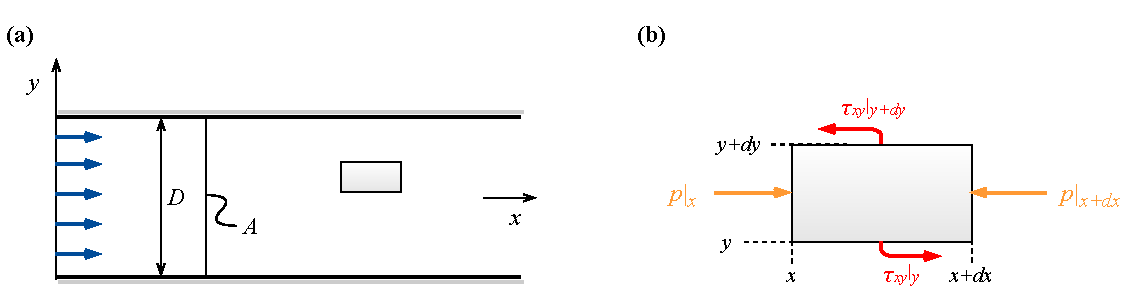
\includegraphics[width=15cm]{plots/poiseuille-flow.pdf}
\caption{Flow between two parallel plates with an infinitesimal fluid element.}			
\label{fig:poiseuille-fluid-element}
\end{figure}

We also have three boundary conditions. Due to a no-slip condition we assume that the velocity at the very surface of the plates is zero: $u(-D/2) = 0$ and $u(D/2) = 0$. Due to symmetry of the flow we assume that there cannot be any net momentum transfer between the upper half and the lower half of the channel. Hence, the shear stress exactly in the middle of the channel is zero: $\tau_{xy}(0) = 0$.

Steady state momentum (force) balance, taking into account pressure and shear forces on a single infinitesimal fluid element:

\begin{equation}
0 = p|_x B dy - p|_{x+dx} B dy + \tau_{xy}|_y B dx - \tau_{yx}|_{y+dy} B dx
\end{equation}

Dividing both sides by the width $B$ and by $dx dy$ we obtain:

\begin{equation}
0 = \frac{p|_x  - p|_{x+dx}}{dx}  + \frac{\tau_{xy}|_y  - \tau_{yx}|_{y+dy}}{dy} 
\end{equation}

Now we notice that $\frac{p|_x  - p|_{x+dx}}{dx}$ is in fact equal to $-\frac{dp}{dx}$ (in a limit as $dx \rightarrow 0$), since it is an incremental change in pressure function value per incremental distance $dx$. Similar thing can be said about $\frac{\tau_{xy}|_y  - \tau_{yx}|_{y+dy}}{dy}$ which is equal to $-\frac{d \tau_{xy}}{dy}$. We can thus further simplify:

\begin{equation}
\frac{d \tau_{xy}}{dy} = - \frac{dp}{dx} = \text{const}
\end{equation}

Integrating the above equation and applying the initial condition for the shear stress $\tau_{xy}(0) = 0$:

\begin{equation} \label{eq:shear-poiseuille}
\tau_{xy}(y)= - \frac{dp}{dx} y
\end{equation}

Adding a constitutive relation for Newtonian fluids we can further relate pressure and velocity. From the Newton's law we know also that:

\begin{equation} \label{eq:shear-newton}
\tau_{xy}(y)= - \mu \frac{du}{dy}
\end{equation}

You may look at this in such a way: the equation \ref{eq:shear-poiseuille} is a special case in which the shear stresses have been related to the driving force in the Poiseuille flow - the pressure gradient. The equation \ref{eq:shear-newton} is a general description of any shear stress $\tau_{xy}$, where it is linked to velocity gradients, no matter what the cause for this velocity gradient is! It just so happens that in the case of a Poiseuille flow between two parallel plates this cause is the pressure drop:

\begin{equation}
- \mu \frac{du}{dy} = - \frac{dp}{dx} y
\end{equation}

Integrating one more time the above relation and applying the no-slip boundary conditions we get:

\begin{equation}
u(y) = \frac{1}{2 \mu} \frac{dp}{dx} (y^2 - (D/2)^2)
\end{equation}

